%%%%%%%%%%%%%%%%%%%%%%%%%%%%%%%%%%%%%%%%%
% Stylish Article
% LaTeX Template
% Version 2.1 (1/10/15)
%
% This template has been downloaded from:
% http://www.LaTeXTemplates.com
%
% Original author:
% Mathias Legrand (legrand.mathias@gmail.com) 
% With extensive modifications by:
% Vel (vel@latextemplates.com)
% Final ACS by:
% Juan Barbosa
% License:
% CC BY-NC-SA 3.0 (http://creativecommons.org/licenses/by-nc-sa/3.0/)
%
%%%%%%%%%%%%%%%%%%%%%%%%%%%%%%%%%%%%%%%%%
\documentclass[fleqn,10pt]{SelfArx}
%\usepackage[superscript]{cite}
\usepackage{wrapfig}
\usepackage{multirow}
%----------------------------------------------------------------------------------------
%	ARTICLE INFORMATION
%----------------------------------------------------------------------------------------

\JournalInfo{Laboratorio de Bioquímica, No. 2, 11/02/2019} % Journal information
\Archive{ }

\PaperTitle{Determinación de proteínas en huevo y harina de trigo} %
%\Keywords{Keyword1 --- Keyword2 --- Keyword3} % Keywords - if you don't want any simply remove all the text between the curly brackets
%\newcommand{\keywordname}{Keywords} % Defines the keywords heading name

%----------------------------------------------------------------------------------------
%	ABSTRACT
%----------------------------------------------------------------------------------------

\Abstract{
%	The extraction and analysis of biological components such as carbohydrates, lipids and proteins is of vital importance for medicine and biochemistry. Because of this importance, qualitative tests have been developed, such as Lugol, Molish, Saponification, Benedict, Biuret and Ninhydrin, being these the ones studied on this document using animal tissues, to identify the presence of carbohydrates, lipids and proteins in the different samples. In order to isolate these compounds we carried out a tissue fractionation using centrifuge related procedures. Results show the presence of carbohydrates, lipids and proteins in all the studied samples. Nevertheless there are contradicting results associated to specific tests and samples, that made impossible to accurately relate the results from the different tissues.
}

%----------------------------------------------------------------------------------------

\begin{document}

\flushbottom % Makes all text pages the same height

\maketitle % Print the title and abstract box
%\tableofcontents % Print the contents section

\thispagestyle{empty} % Removes page numbering from the first page



%----------------------------------------------------------------------------------------
%	ARTICLE CONTENTS
%----------------------------------------------------------------------------------------

\section*{Introducci\'on} % The \section*{} command stops section numbering
%-----------------------------------------------
	
\section{Secci\'on experimental}
En un balon aforado de 250 mL fueron disueltos 0.38 g de sulfato de cobre (II) pentahidratado, y 1.5 g de tartrato de sofio y potasio tetrahidratado usando 75 mL de una soluci\'on de hidr\'oxido de sodio 10 \% preparada previamente. Posteriormente fue adicionado 0.25 g de yoduro de potasio y finalmente, la soluci\'on aforada. En un balón aparte fueron disueltos 1 g de cloruro de sodio en 100 mL de agua.
	\subsection{Preparaci\'on de la muestra}
		Cerca de 2 g de harina fueron disueltas en 10 mL de cloruro de sodio al 1 \%. La muestra disuelta fue centrifugada por 10 minuto a 2800 rpm. El sobrenadante fue aforado en 25 mL de de la soluci\'on de NaCl. En el caso de la clara de huevo, se realiz\'o una primera diluci\'on 1:10 usando cloruro de sodio al 10 \% en un bal\'on de 25 mL. Posteriormente se realizaron dos diluciones de 1 en 5, y 1 en 10, con NaCl en balones de 25 mL.
		
	\subsection{Preparaci\'on de las soluciones stock}
		Para el estudio de la prote\'ina en la harina, se prepar\'o una soluci\'on stock con concentraciones de 2.5 mg/mL de alb\'umica s\'erica y 2.5 mg/mL de globulina. Para la soluci\'on stock asociada con la alb\'umina de huevo, se pesaron 50 mg de ovoalb\'umina, los cuales fueron aforados en 10 mL de agua.

	\subsection{Curvas de calibraci\'on y medidas}
		Los patrones de las curvas de calibraci\'on fueron preparados realizando diluciones de 0.0, 0.2, 0.4, 0.8, 1.2, 1.6 y 2.0 mL de cada soluci\'on stock en 8 mL del reactivo de Biuret previamente preparado. De forma an\'aloga, se tomaron 2.0 mL de las soluciones de harina y huevo, las cuales se aforaron en balones de 10 mL usando el reactivo de Biuret. Todas las soluciones se dejaron reposar por cerca de 30 minutos, hasta observar que las muestras manten\'ian un color constante.
		
		Se construyeron las curvas de calibraci\'on a 571 nm usando celdas de pl\'astico y la soluci\'on de cloruro de sodio, previamente preparada, como blanco.
	
\section{Resultados y Discusi\'on}

	En el caso de la alb\'umina de huevo, se realizaron dos diluciones a partir de una primera soluci\'on stock de 1:10 clara de huevo : NaCl (ac) 1 \%. La primera de estas corresponde con una disoluci\'on 1:10, y la segunda 1:5, las concentraciones calculadas a partir de las absorbancias reportadas por los distintos grupos de laboratorio, y sus curvas de calibraci\'on se muestran en la \autoref{tb: huevo_concentraciones}. Con el objetivo de determinar si los datos son suficientemente coherentes para la realizaci\'on de un an\'alisis estad\'istico entre grupos, para determinar el intervalo de confianza, se realiza la raz\'on entre la concentraci\'on obtenida para las disoluciones antes mencionadas, para la cual se deber\'ia obtener un factor de 2. Sin embargo, como se observa en la \autoref{tb: huevo_concentraciones}, no se evidencia ninguna relaci\'on constante para todos los 5 grupos, de hecho, los factores se pueden agrupar en 3 subgrupos: 1.15, $\approx$ 1.75 y $\approx$ 2.5. La presencia de 3 subgrupos en una muestra de 5, ocasiona que exista al menos 1 grupo con un \'unico dato, haciendo poco confiable un estudio estad\'istico, dada el taman\~o de la muestra.
	\begin{figure*}[h]
		\centering
		\begin{tabular}{cc}
			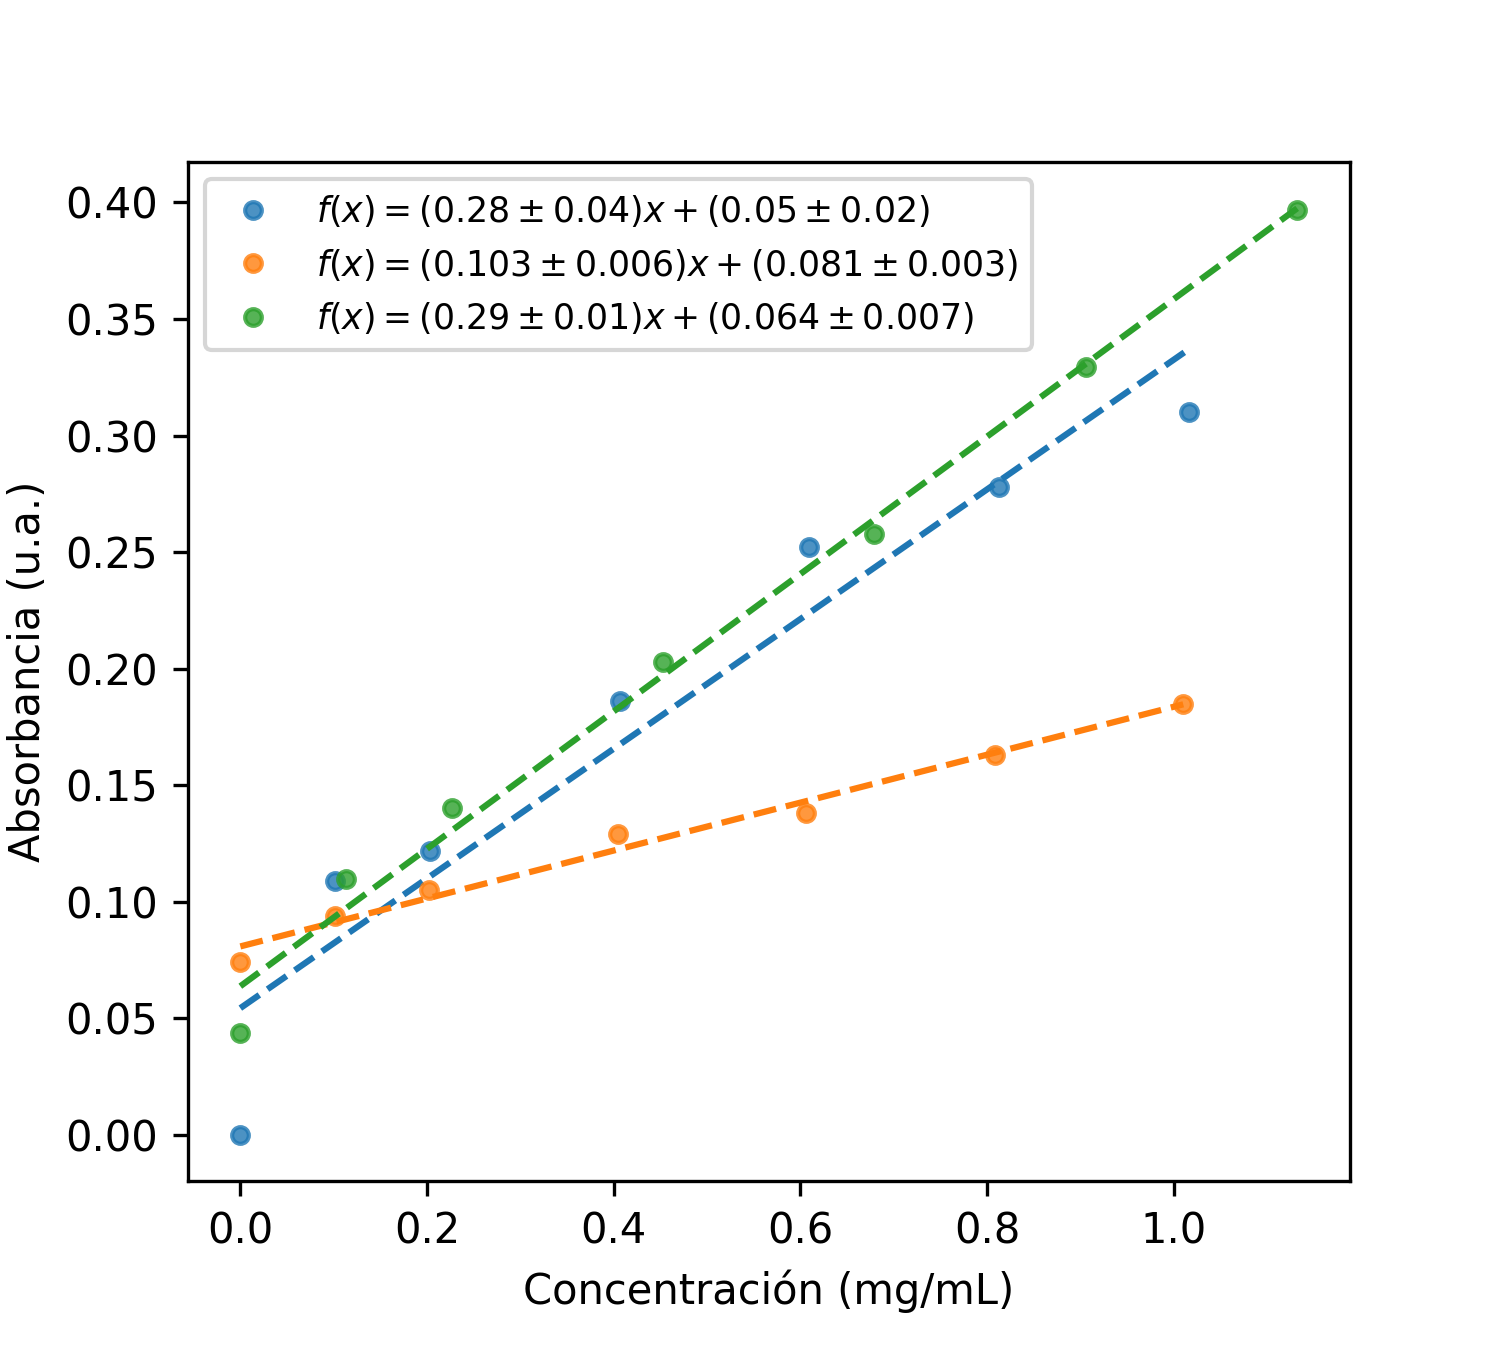
\includegraphics[width = 0.45\linewidth]{harinas_reg} & 
			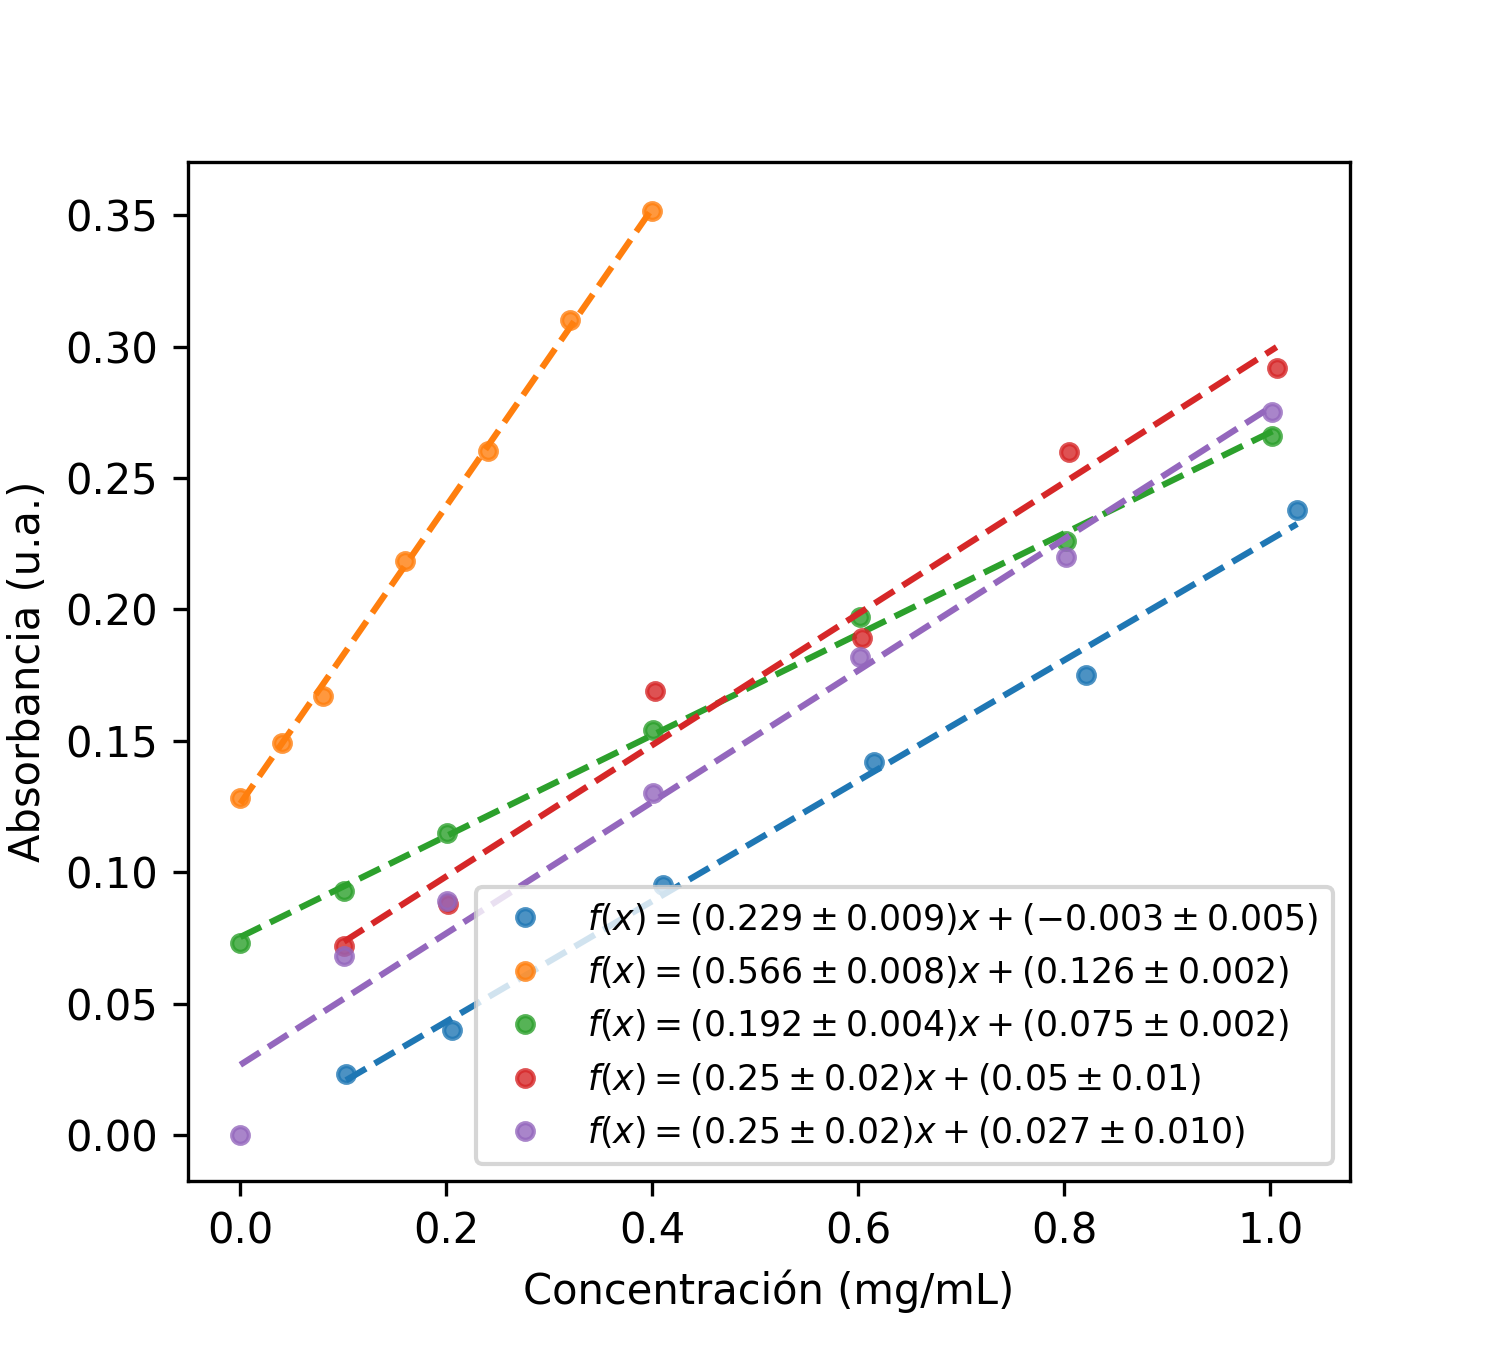
\includegraphics[width = 0.45\linewidth]{huevos_reg}
		\end{tabular}
		\caption{Curvas de calibraci\'on para la harina (izquierda) y huevo (derecha).}
		\label{fig: pendientes}
	\end{figure*}

	\begin{table}[h]
		\centering
		\caption{Concentraciones obtenidas para las dos diluciones de la soluci\'on stock medidas del huevo.}
		\label{tb: huevo_concentraciones}
		\begin{tabular}{c|cc|c}
			\hline
			\textbf{Grupo} & \textbf{1:10 (mg/mL)} & \textbf{1:5 (mg/mL)} & \textbf{Raz\'on} \\
			\hline
			1 & 1.7205 & 1.9869 & 1.15 \\
			2 & 0.0809 & 0.1979 & 2.45 \\
			3 & 0.2222 & 0.5711 & 2.57 \\
			4 & 0.7040 & 1.2596 & 1.79 \\
			5 & 0.3649 & 0.6327 & 1.73 \\
			\hline
		\end{tabular}
	\end{table}

	Para reportar el valor esperado de la prote\'ina del huevo con alg\'un intervalo de confianza, es necesario conocer a profundidad la distribuci\'on de los datos. En la \autoref{fig: dist} se muestra c\'omo se distribuyen las concentraciones inferidas para la ovoalb\'umina, mostrando que existe informaci\'on insuficiente para determinar la distribuci\'on real de la muestra, por otro lado el corrimiento horizontal para datos de un mismo color (grupo), resalta el argumento anterior de una falta de coherencia en la informaci\'on reportada. Esto \'ultimo es de particular importancia dado que se puede argumentar que dos huevos extra\'idos de ambientes completamente distintos han de tener una concentraci\'on de prote\'ina diferente, si bien los autores consideran este argumento como v\'alido, para un mismo grupo \'este carece de aplicaci\'on, por lo cual, la disperci\'on en la concentraci\'on obtenida deber\'ia ser considerablemente menor.
	\begin{figure}[h]
		\centering
		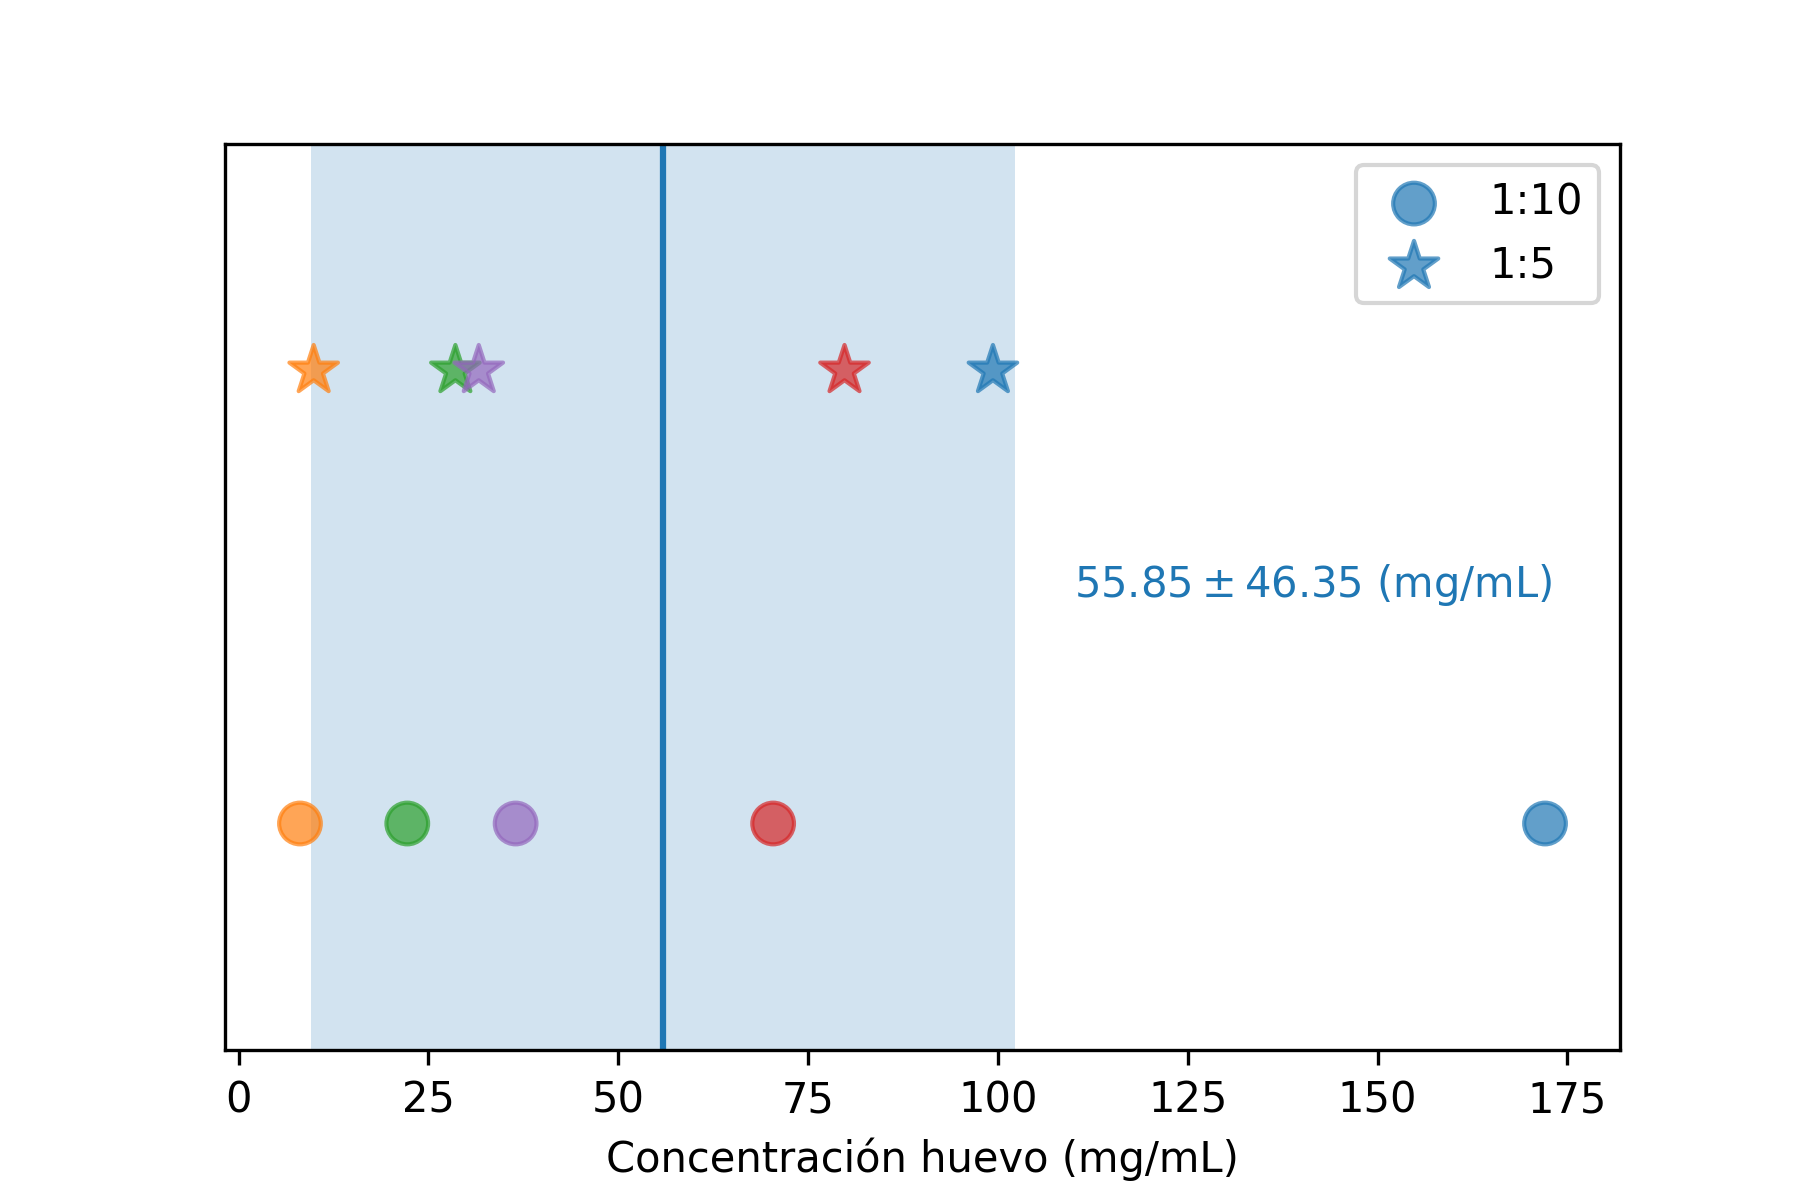
\includegraphics[width=\linewidth]{concentraciones}
		\caption{Distribuci\'on de la concentraci\'on prote\'inas en la clara de huevo a partir de los datos. Usando c\'irculos se muestran las concentraciones inferidas a partir de las disoluciones 1:10, cada color se encuentra asociado a las pendientes de la \autoref{fig: pendientes}. La l\'inea azul muestra el promedio de los datos, y el \'area coloreada la regi\'on entre $\mu \pm \sigma$.}
		\label{fig: dist}
	\end{figure}

	A pesar de las incongruencias antes mencionadas, se reporta la concentraci\'on de ovoalb\'umina en la clara de huevo en $(5\pm4)\times10^{1}$ mg/mL. Dos posibles explicaciones a los resultados son propuestas, por un lado, la preparaci\'on de la muestra del huevo es considerablemente m\'as compleja que para la harina, esta complejidad puede explicar los disperci\'on de los resultados entre grupos. En el caso de los valores obtenidos para un mismo grupo, existe la posibilidad que la reacci\'on de las prote\'inas con el reactivo de Biuret no haya llego a su fin, y lo que se observa sea un efecto cin\'etico, en la que unas muestras hayan progresado m\'as en la reacci\'on que otras. 

\section{Conclusiones}
	
%----------------------------------------------------------------------------------------
%	REFERENCE LIST
%----------------------------------------------------------------------------------------
\phantomsection
\bibliography{informe}
\bibliographystyle{unsrt}

%----------------------------------------------------------------------------------------
%\newpage
%\onecolumn
%\section{Informaci\'on suplementaria}\label{sec: complementaria}
\end{document}